\section{类\texttt{class}初步}
{\kaishu\large ``一个设计良好的类能为用户提供简洁易用的接口\footnote{接口(Interface),在信息技术中指能将不同部件连接起来的媒介。通过接口,不同部件之可以进行信息交换。例如,笔记本电脑有USB接口,如果手机通过数据线连到这个接口上,那么笔记本电脑就可以和手机交换信息。},并将其内部结构隐藏起来,用户根本不必了解其内部结构。如果内部结构不应该被隐藏——例如,因为用户需要随意改变类中的任何数据成员——你可以把这种类认为是`普通的老式数据结构'。''\footnote{原文:A well-designed class presents a clean and simple interface to its users, hiding its representation and saving its users from having to know about that representation. If the representation shouldn't be hidden - say, because users should be able to change any data member any way they like - you can think of that class as `just a plain old data structure'.}}
\begin{flushright}——比雅尼·斯特劳斯特鲁普\end{flushright}\par
我们在第二节中所介绍的结构体更接近于C风格。它只能实现``把多个数据包装到一个对象中''的功能。而在使用时,我们可以任意地改变它的成员变量。这样做的好处是方便,简单,直接。如果我们要写一个结构体来管理单链表,我们完全可以这样写:
\begin{lstlisting}
struct List {
    struct Data { //在List内部定义Data类
        int num;
        Data *next;
    };
    Data head; //Data类的成员head
};
\end{lstlisting}
接下来我们只要用它就行了。\par
但是当我们要用这个单链表时,那就有些麻烦了:\par
我们必须知道这个链表是怎么实现的,并且亲自去修改它的成员。为了解决这个问题,我们尚且可以写一些函数来针对 \lstinline@struct@ 的成员进行修改。\par
结构体对外不封闭,程序员可以随意更改成员变量的值。这就会带来安全性问题,我们不能防止自己或别人因为各种原因(失误也好,有意操作也罢)乱改结构体的成员(尤其是乱改指针的值,指针可不是闹着玩的)。\par
C++大大扩展了 \lstinline@struct@ 的能力,并引入了关键字 \lstinline@class@ 作为 \lstinline@struct@ 的替代\footnote{\lstinline@class@ 与 \lstinline@struct@ 只有两个方面的不同:其一,\lstinline@class@ 的默认成员访问权限是 \lstinline@private@,而 \lstinline@struct@ 的默认成员访问权限是 \lstinline@public@;其二,\lstinline@class@ 的默认继承方式是 \lstinline@private@,而 \lstinline@struct@ 的默认继承方式是 \lstinline@public@。除此之外,\lstinline@class@ 和 \lstinline@struct@ 没有任何本质差异。}。\par
\subsection*{类的成员访问权限}
在普通的老式数据结构中,所有的成员都毫无保留地公开,外界可以任意地读取或修改它;而在类中,我们会把成员的访问权限分成三种:
\begin{itemize}
    \item \lstinline@public@ 公有成员。它们是对外公开的,外界可以访问。
    \item \lstinline@private@ 私有成员。它们对外不公开,外界无法访问。只有类中的其它成员\footnote{一般是成员函数,见下文。}才能访问或修改它。外界如果想要访问它,只能以 \lstinline@public@ 成员作为中介。
    \item \lstinline@protected@ 受保护成员。它们对外不公开,但对派生类\footnote{我们会在第九章介绍相关内容。}公开。
\end{itemize}
\lstinline@private@ 成员是类与老式数据结构的关键区别。通过 \lstinline@private@ 成员,我们可以将类的一些内部结构隐藏起来,只有这个类中的其它成员能够访问。\par
举例来说,\lstinline@istream@ 就是一个类,我们一直在使用它的一个名为 \lstinline@cin@ 的对象。这个 \lstinline@istream@ 类的内部结构是怎样的?它如何把我们的输入信息解释出来,并且赋值给右操作数?它如何记标输入异常状态?这些内容纷繁复杂,C++自有它的实现机制。\par
但是我们不用考虑这么多!我们只需要在输入的时候写一个 \lstinline@cin>>num@ 就行了;如果要清理输入异常,我们直接调用成员函数 \lstinline@clear()@ 就够了!C++把底层的实现机制放到 \lstinline@private@ 成员中,而 \lstinline@public@ 成员则是它对外的接口,我们用的 \lstinline@clear@ 就是一个 \lstinline@public@ 成员\footnote{至于 \lstinline@>>@,它不是 \lstinline@istream@ 的成员。它使用了友元,我们会在第八章介绍这些内容。}。图6.11体现了这两种对象的关系。\par
\begin{figure}[htbp]
    \centering
    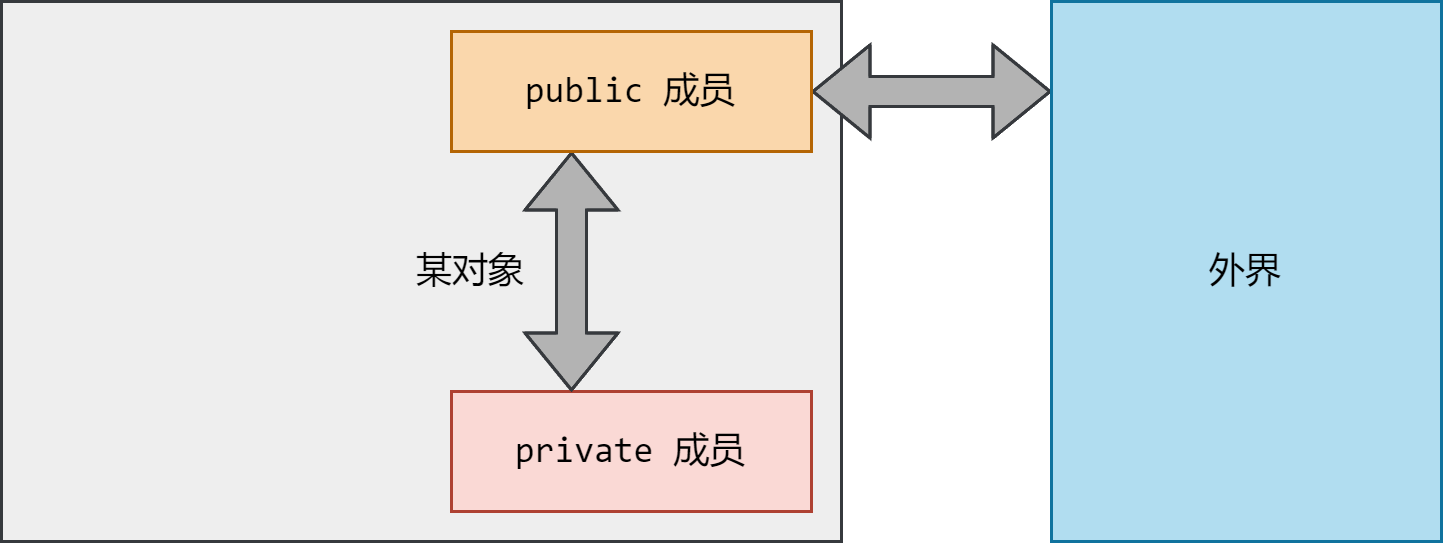
\includegraphics[width=0.6\textwidth]{../images/generalized_parts/06_public_and_private_members.drawio.png}
    \caption{\lstinline@public@ 成员提供对外界的接口,而 \lstinline@private@ 成员隐藏了底层的细节}
\end{figure}
至于 \lstinline@protected@ 成员,在不涉及继承时,它和 \lstinline@private@ 成员没什么区别,我们可以暂时把它当作 \lstinline@private@ 成员来看待。\par
举个例子,\lstinline@string@ 库中的 \lstinline@string@ 类\footnote{实际上它是 \lstinline@basic_string@ 类的一个实例,我们暂时不讨论这些细节问题,把 \lstinline@string@ 当成一个类即可。}提供了强大的字符串存储和处理功能,比如说它可以动态地改变字符串的容量,用 \lstinline@=@ 直接为字符串赋值,以及用 \lstinline@+=@ 拼接字符串等。
\begin{lstlisting}
    string str {"Bjarne Stroustrup"}; //需要头文件string
    str = "Donald Ervin Knuth"; //可以用等号赋值!
    cout << str << endl; //将输出Donald Ervin Knuth
    str = "Alexander Alexandrovich"; //str会动态改变长度,不怕越界
    cout << str << endl; //将输出Alexander Alexandrovich
    str += " Stepanov"; //用+=运算符拼接
    cout << str << endl; //将输出Alexander Alexandrovich Stepanov
    cout << str.length(); //输出str当前的长度,应为32
\end{lstlisting}\par
这里的赋值 \lstinline@=@、加赋值 \lstinline@+=@ 和 \lstinline@length@ 都是在 \lstinline@string@ 类中定义的成员函数,它们是公有成员,我们可以直接使用;而这个类的底层实现是通过动态内存分配和各种成员变量来记录的,它们是私有成员,我们必须通过公有成员来找到它们。就以 \lstinline@length@ 成员函数为例吧,它是一个公有成员,在 \lstinline@basic_string@ 中的定义是这样的:
\begin{lstlisting}
public:
    _NODISCARD _CONSTEXPR20 size_type length() const noexcept {
        return _Mypair._Myval2._Mysize;
    }
\end{lstlisting}
函数体中给出了它的返回值 \lstinline@_Mypair._Myval2._Mysize@,这是什么呢?再查,会发现 \lstinline@_Mypair@ 定义在这里:
\begin{lstlisting}
private:
    _Compressed_pair<_Alty, _Scary_val> _Mypair;
\end{lstlisting}
至于这个 \lstinline@_Mypair@ 具体是什么,我们就不多追究了,总之它的某个叫做 \lstinline@_Myval2._Mysize@ 的成员存储了这个长度信息。\par
再来看它们的访问权限。我们会发现,\lstinline@length@ 是公有(看到那个 \lstinline@public@ 了吗)成员,而 \lstinline@_Mypair@ 是私有(看到那个 \lstinline@private@ 了吗)成员。这就说明,我们可以调用 \lstinline@length@ 来返回 \lstinline@_Mypair._Myval2._Mysize@,但不能直接用这个私有成员。这样就非常安全,外界不能任意篡改 \lstinline@_Mypair@;而且也非常方便,我们根本就不需要知道 \lstinline@_Mypair._Myval2._Mysize@ 这个复杂的用法,只需要调用成员函数 \lstinline@length@ 就够了。\par
而在调用其它成员函数,比如赋值运算符时,这个字符串的长度值也可能发生变化。下面是 \lstinline@assign@\footnote{实际调用赋值运算符时都要经过 \lstinline@assign@ 这一步,我们就不多说了。}函数的实现,读者只需关注 \lstinline@_Mypair._Myval2._Mysize=_Count@ 这一步,它就是一个改变长度的过程。
\begin{lstlisting}
public:
    _CONSTEXPR20 basic_string& assign(
        _In_reads_(_Count) const _Elem* const _Ptr, _CRT_GUARDOVERFLOW
        const size_type _Count) {
        if (_Count <= _Mypair._Myval2._Myres) {
            //...
            _Mypair._Myval2._Mysize = _Count; //在这里改变了长度值
            //...
\end{lstlisting}
\subsection*{类的成员函数}
以往我们的函数都是定义在全局范围内的。C++允许我们在类中定义函数,这样的函数叫作\textbf{成员函数(Member function)}。上文讲到的 \lstinline@length@ 就是 \lstinline@string@ 类的一个成员函数。\par
成员函数的特点有二:其一,成员函数只能由这个类的对象来调用;其二,成员函数可以访问这个类的 \lstinline@protected@/\lstinline@private@ 成员。\par
假如说我们想要模仿 \lstinline@string@ 类的思路来写一个简易版本的 \lstinline@String@ 类,我们可以这么写:
\begin{lstlisting}
class String { //String类的定义
public: //从这里开始的都是公有成员
    unsigned length() { //返回值表示str的长度
        return _length; //String类的成员可以访问私有成员_length
    }
    void assign(const char *src) { //改变str字符串中的内容
        strncpy(_str, src, 100); //String类的成员可以访问私有成员_str
        _length = strlen(_str); //更新_length的值
    }
private:
    char _str[100]; //实际的string使用指针和动态内存分配,这里简化成用char[100]
    unsigned _length; //私有成员_length,用来记录现在str的长度
};
\end{lstlisting}
在这里我们定义了 \lstinline@String@ 类的部分功能,包括两个公有成员函数和两个私有成员变量。接下来我们解释一下它们的作用。\par
\lstinline@_length@ 私有变量用于记录现在 \lstinline@_str@ 中存储的有效内容的长度,这个不难理解。而 \lstinline@length()@ 函数用于返回这个值。这样我们定义的任何 \lstinline@String@ 类变量都可以通过 \lstinline@length()@ 成员函数来返回它的值。
\begin{lstlisting}
    String str1; //这里不能再用结构体那种初始化语法了,我们之后再谈
    cout << str1.length(); //用成员访问运算符.访问length()成员函数
\end{lstlisting}
\lstinline@_str@ 是一个数组,我们可以用它来存储一串字符。但 \lstinline@_str@ 是一个私有成员,我们不能直接修改它,因此 \lstinline@assign@ 公有成员函数就派上用场了。
\begin{lstlisting}
    String str2; //再定义一个str2
    str2.assign("Bjarne Stroustrup"); //由str2调用assign
\end{lstlisting}
在 \lstinline@str2@ 调用 \lstinline@assign@ 的时候,程序会把 \lstinline@"Bjarne Stroustrup"@ 作为 \lstinline@const char*@ 数据传给 \lstinline@assign@ 函数\footnote{实际被传递的还有 \lstinline@&str2@,作为隐藏参数 \lstinline@this@ 传递。详见第八章。}。在函数调用期间,\lstinline@strncpy@ 会改变私有成员 \lstinline@_str@ 的内容,而 \lstinline@strlen@ 会计算 \lstinline@_str@ 的有效长度并以此改变 \lstinline@_length@。\par
初学者,尤其是从C语言过渡到C++的学习者,往往会觉得 \lstinline@class@ 这种设置访问权限的写法实在是太麻烦了,还不如 \lstinline@struct@ 那样一切默认用 \lstinline@public@ 的方法好。这种想法对于小规模的工程来说还好,但是对于大规模的工程来说,如果没有成员函数加以封装,没有私有访问权限加以保护,那么我们很容易在复杂的工程中写很多冗余代码,或者是犯一些低级错误。这就像是我们用函数——我们当然可以不用函数,但用了函数能让我们的生活更轻松;或者像是我们用 \lstinline@const@——我们当然可以不用 \lstinline@const@,只要你能确保自己写代码时不犯误修改某个值的错误。但是我们还是会选择用它们,也会选择用 \lstinline@class@ 代替 \lstinline@struct@,道理也是一样的。等到读者有了更多的编码经验之后,想必也会体会到这一点。\par
\subsection*{\texttt{vector}简介与示例}
C++中有一个动态数组类模板 \lstinline@vector@,它定义在头文件 \lstinline@vector@ 中,是STL的一部分。我们暂时不讲STL,但可以以它为例,讲一下类的成员函数的应用。
它是一个类模板,我们需要指定具体的类型,比如 \lstinline@int@ 或者 \lstinline@double@,从而让它变为一个类实例。为了避免过多无关信息干扰读者的思路,我们直接这么写吧:
\begin{lstlisting}
#include <vector> //包含头文件vector
using vecint = vector<int>; //vecint相当于vector<int>类的别名
\end{lstlisting}
接下来我们可以直接用 \lstinline@vecint@ 作为 \lstinline@vector<int>@ 类的别名,所以 \lstinline@vecint@ 就成了一个类型。这样理解就好。\par
\lstinline@vecint@ 有一个成员函数 \lstinline@push_back@,它允许我们每次向这个动态数组中添加一个元素;还有一个成员函数 \lstinline@size@,它的返回值是当前数组的有效数字个数。
\begin{lstlisting}
    vecint v; //定义一个v,这时它的有效数字个数为0
    for (int i = 0; i < 10; i++) {
        v.push_back(i); //每次向v中添加数据
        std::cout << v.size() << ' '; //每次输出v的有效数字个数
    }
\end{lstlisting}
这个程序的输出如下:\\\noindent\rule{\linewidth}{.2pt}\texttt{
1 2 3 4 5 6 7 8 9 10
}\\\noindent\rule{\linewidth}{.2pt}\\
不难看出,这个动态数组的数据量是在变化的。\par
\lstinline@vecint@ 有一套动态调整容量的机制,如果要存储的数据量超过了原有的容量(比如说,用 \lstinline@push_back@ 向已满的数组中添加新数据),它就会重新分配一块更大的内存空间。我们可以用 \lstinline@capacity@ 函数来输出 \lstinline@v@ 的容量。
\begin{lstlisting}
    vecint v; //定义一个v,这时它的容量为0
    for (int i = 0; i < 20; i++) {
        v.push_back(i); //添加数据,如果数据量超过了容量,v将会自动扩容
        std::cout << v.capacity() << ' '; //输出v的当前容量。
    }
\end{lstlisting}
这个程序的输出如下:\\\noindent\rule{\linewidth}{.2pt}\texttt{
1 2 3 4 6 6 9 9 9 13 13 13 13 19 19 19 19 19 19 28
}\\\noindent\rule{\linewidth}{.2pt}\\
也不难看出,随着我们不断向 \lstinline@v@ 中添加数据,它的容量会以一种特殊的方式来扩充——不是每次加一(重新分配内存会很浪费时间)。\par
如果我们预先知道我们需要多少容量,我们也可以用 \lstinline@reserve@ 函数一次性分配这么大的容量。\footnote{\lstinline@reserve@ 的作用是,如果现在的容量小于 \lstinline@reserve@ 的参数中给定的值,就把它的容量扩充到这个值;否则就什么也不做。}
\begin{lstlisting}
    vecint v; //定义一个v,这时它的容量为0
    v.reserve(50); //用reserve改变其容量
    for (int i = 0; i < 50; i++)
        cin >> v.at(i); //向数组中输入值
\end{lstlisting}\par
这里的 \lstinline@v.at(i)@ 有点像是数组下标访问的形式,它也是从 \lstinline@0@ 开始的,所以 \lstinline@v.at(i)@ 对应的是数组的第 \lstinline@i+1@ 个数。实际上 \lstinline@vecint@ 重载了下标运算符,它使得我们可以用更简单的方式来表达 \lstinline@v.at(i)@。\par
\begin{lstlisting}
    for (int i = 0; i < 50; i++)
        cin >> v[i]; //直接用下标来访问,就像真的数组一样
\end{lstlisting}\par
这些功能看上去让人眼花瞭乱,但它们的思路都不难想,我们有了一定的基础之后也可以自己写一个低配版的 \lstinline@vecint@ 出来。在后面的章节中我们会实操一些相关方面的内容,比如实现 \lstinline@vector@, \lstinline@valarray@, \lstinline@string@ 和 \lstinline@stack@ 等——看上去很吓人,但实际上没有那么难。当读者把这些代码的构建全部练过一遍之后,读者对C++的理解想必会更上一层楼。\par
不过莫急,我们先插叙一章,来讲讲代码工程的相关知识。\par
34